\documentclass[UTF8]{ctexart}
\usepackage{graphicx}
\usepackage{subfigure}
\usepackage{amsmath}
\usepackage{geometry}
\usepackage{enumerate}
\usepackage{cite}
\usepackage{booktabs}
\usepackage{listings}
\usepackage{color}
\usepackage{xcolor}
\usepackage{titletoc}

\lstset{language=C++}
\lstset{breaklines}%这条命令可以让LaTeX自动将长的代码行换行排版
\lstset{extendedchars=false}%这一条命令可以解决代码跨页时,章节标题,页眉等汉字不显示的问题

\geometry{left=2cm,right=2cm,top=2cm,bottom=2cm}

\title{\heiti 《计算空气动力学》 \\ 大作业}
\author{SX1501021 仓宇}
\date{\today}

\bibliographystyle{plain}

\begin{document}
\maketitle
\setcounter{page}{0}
\thispagestyle{empty}
\clearpage

\tableofcontents
\clearpage

\section{问题描述}
求解无粘条件下NACA0012翼型的2维平面流场。流场网格是由三角形单元组成的非结构网格,使用有限体积方法求解流场的2维Euler方程。网格文件为data文件夹下的naca0012.grd文件。全流场的网格如下左图所示,右图是翼型周围的网格:
\begin{figure}[htbp]\centering
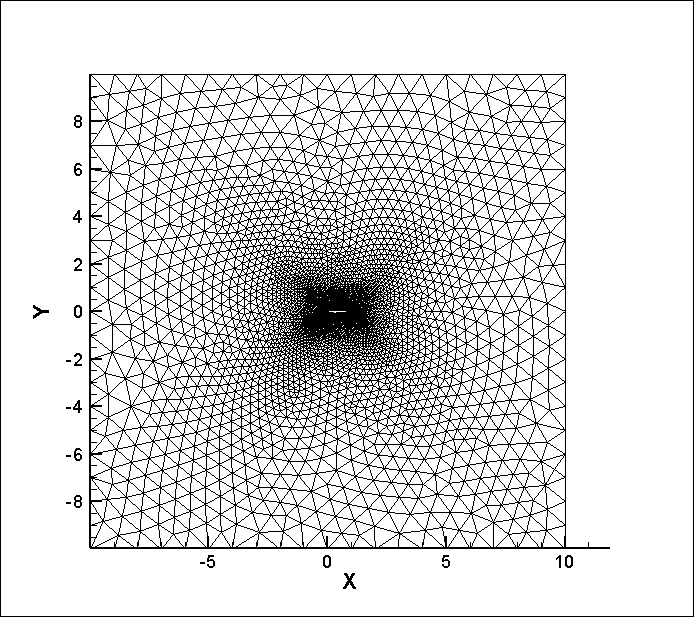
\includegraphics[width=5.5cm,height=4.5cm]{../data/mesh_naca0012.png}
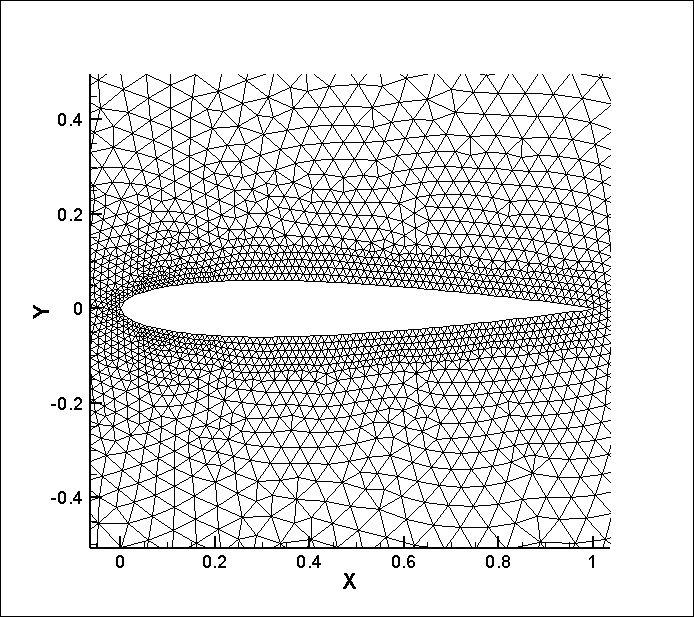
\includegraphics[width=5.5cm,height=4.5cm]{../data/mesh_naca0012_local.png}
\caption{用于NACA0012翼型的非结构网格}
\end{figure}

\section{问题分析}
本文采用Jameson中心格式来求解二维Euler方程。在空间离散上采用的是有限体积法,时间上采用的是四步显式Runge-Kutta迭代求得最后的定常解。人工耗散项为守恒变量的二阶和四阶差分项。边界条件采用的是无反射边界条件,并采用当地时间步长进行加速收敛。

\subsection{基本方程}
由于不考虑粘性,二维NS方程可简化为Euler方程。欧拉方程是质量,动量,能量守恒定理的表达。在边界为S,面积为Ω的二维区域,方程可以写成以下形式:
\begin{equation}\label{euler}
\frac{\partial}{\partial t} \iint_{\Omega} W d\Omega + \int_{S} (Fdy-Gdx) = 0
\end{equation}

\indent 其中,$x,y$是笛卡尔坐标,$W$是守恒量矢量,$F,G$是流动矢量,具体形式如下:
\begin{equation}
W={\begin{bmatrix} \rho \ \rho U \ \rho V \ \rho E \end{bmatrix}}^\mathrm{T}
\end{equation}

\begin{equation}
F={\begin{bmatrix} \rho U \ \rho U^2 + P \ \rho UV \ \rho UH \end{bmatrix}}^\mathrm{T}
\end{equation}

\begin{equation}
G={\begin{bmatrix} \rho V \ \rho UV \ \rho V^2 + P \ \rho VH \end{bmatrix}}^\mathrm{T}
\end{equation}

\indent $\rho,P,H,E$分别是密度,压强,单位质量总焓和单位质量总能量;$U,V$是速度矢量的笛卡尔坐标系下的分量。这些变量之间的关系如下:
\begin{equation}
\rho E=P/(\gamma-1)+\rho (U^2+V^2)/2
\end{equation}

\begin{equation}
\rho H=\rho E + P
\end{equation}

\subsection{空间离散}
计算区域被划分为有限数量的非重叠单元,并且积分形式的守恒方程应用到每个单元。单元的一般形状如下图所示:
\begin{figure}[htbp]\centering\label{cell}
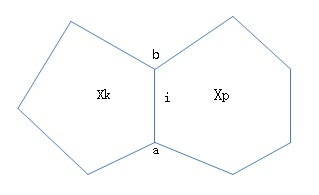
\includegraphics[width=6.5cm,height=4.5cm]{../data/cell.jpg}
\caption{离散的单元示意图}
\end{figure}

\indent 因为考虑到时间,任何单元的体积都可视作常数,所以\eqref{euler}可写成如下形式:
\begin{equation}\label{discrete}
\frac{\partial W}{\partial t} = - \frac{\int_S (Fdy-Gdx)}{\iint_{\Omega} d\Omega}
\end{equation}

\indent 对于任一单元k,\eqref{discrete}可写成如下形式:
\begin{equation}\label{cell_discrete}
\frac{\partial W_k}{\partial t} = - \frac{Q_k}{\Omega_k}
\end{equation}

\indent 其中,$\Omega_k, W_k, Q_k$分别是单元k的面积、守恒量矢量和\eqref{discrete}右边部分流动积分的离散近似值。\\
\indent $\Omega_k$在网格输入文件中给出,$Q_k$由以下近似给出:
\begin{equation}\label{Q_k}
Q_k=\sum_{i=1}^{edgeNum} (Fdy-Gdx)_i 
\end{equation}

\indent $dx,dy$为每边在坐标轴上的分量,按右手定则确定每条边的正方向,$a,b$分别为每条边的起点和终点,计算规则如下:
\begin{equation}
dx_i=x_b-x_a 
\end{equation}
\begin{equation}
dy_i=y_b-y_a
\end{equation}

\indent 为了计算出每条边上的流动矢量$F,G$,需要知道该边上的守恒量$W_i$,$W_i$由下式近似计算得到:
\begin{equation}\label{W_i}
W_i=(W_k+W_p)/2
\end{equation}

\indent \eqref{W_i}中的$W_k,W_p$分别为Fig\ref{cell}中的左右单元中心处的守恒矢量,从中也可见边的正方向的定义。\\
\indent 为了在计算过程中避免重复计算,我们引入如下辅助变量:
\begin{equation}\label{aid_var}
Z_i=U_i dy_i - V_i dx_i
\end{equation}

\indent 对任一单元k,式\eqref{cell_discrete}可写成如下形式:
\begin{equation}
\frac{\partial W_k}{\partial t} = - \frac{1}{\Omega_k} \sum_{i=1}^{edgeNum}
 {\begin{bmatrix} \rho Z \ \rho UZ+Pdy \ \rho VZ-Pdx \ \rho HZ \end{bmatrix}}^\mathrm{T}
\end{equation}

\indent 对于非结构网格,从边的角度入手来计算每个单元上的守恒矢量的变化量能避免重复计算,且对于网格形状来说具有通用性。

\subsection{人工耗散}

上述单元中心方案是非耗散的,所以任何误差(耗散误差,round-off误差)是没有被考虑进去的,并且振动可能在稳态解中出现。为了消除这些振动,人工耗散项被添加到式\eqref{cell_discrete}的右边部分,对于单元k,式\eqref{cell_discrete}变成如下形式:

\begin{equation}\label{aritificial_dissipation}
\frac{\partial W_k}{\partial t} = - \frac{(Q_k-D_k)}{\Omega_k}
\end{equation}

\indent 在现行工作中,$D_k$被构建成保守变量$W_k$二阶微分和四阶微分的混和。$W_k$的四阶微分的部分被加到平滑的流动区域,但在有激波的区域不起作用,此时$W_k$的二阶微分项被接通用来抑制激波周围的振动,这项可以是相当大的。这种转换通过基于当地压强的二阶微分的激振感应器来获得。$D_k$的计算方法如下:

\begin{equation}
D_k=\sum_{i=1}^{edgeNum}d_{i}^{(2)}+\sum_{i=1}^{edgeNum}d_{i}^{(4)}
\end{equation}

\indent 对于非结构网格,每条边上的保守变量的二阶和四阶微分由下式计算:

\begin{equation}
d_{i}^{(2)}=\alpha_i \varepsilon_{i}^{(2)} (W_p-W_k)
\end{equation}

\begin{equation}
d_{i}^{(4)}=-\alpha_i \varepsilon_{i}^{(4)} (\nabla^{2}W_p-\nabla^{2}W_k)
\end{equation}

\indent 在这里指标i是划分单元k和p的边,$\nabla^{2}W_k$由下式计算得出:

\begin{equation}
\nabla^{2}W_k=\sum_{j=1}^{edgeNum}(W_j-W_k)
\end{equation}

\indent 这里$W_j$指的是与单元k相邻的单元上的守恒矢量,而不是单元k的边界上的守恒矢量。\\
\indent 在现今的工作中,$\varepsilon_{i}^{(2)}$和$\varepsilon_{i}^{(4)}$由如下的一种简单方式构造得出:

\begin{equation}
\varepsilon_{i}^{(2)}=k^{(2)}\nu_i
\end{equation}

\begin{equation}
\varepsilon_{i}^{(4)}=\max(0,k^{(4)}-\varepsilon_{i}^{(2)})
\end{equation}

\indent 这里$k^{(2)}$和$k^{(4)}$是两个由经验得出的常数,数值的典型范围是$1/256<k^{(2)}<1/32$和$1/2<k^{(4)}<10$。\\
\indent $\nu_i$是激振感应器,$\alpha_i$是缩放比例因子,在现今的工作中,激振感应和缩放比例因子在边的基础上构造,只使用两个相邻单元k和p的流动变量,计算形式如下:

\begin{equation}
\nu_i=\frac{\left|P_p-P_k\right|}{\left|P_p+P_k\right|}
\end{equation}

\begin{equation}\label{suofangyinzi}
\alpha_i=\left|Udy-Vdx\right|+c\sqrt{{dx}^2+{dy}^2}
\end{equation}

\indent 这里U,V和c分别是分界边上的速度与当地声速。\\
\indent 在边界附近(有效边界和外边界)对耗散项不正确的处理将导致解精度的严重损失。添加用来抑制振动的耗散项可以变得过于强,局部地,数值方案的顺序可被简化。从物理的观点来看,这种强耗散在边界附近产生了大量的伪数值熵。这引起了翼型表面的压强损失,而且积分载荷也会不正确。

\subsection{时间离散}
稳态解是通过对大系统的常微分方程的时间积分所得到的,可以写成如下形式:
\begin{equation}\label{time_discrete}
\frac{dW_k}{dt}=-\frac{Q_k-D_k}{\Omega_k} \equiv R_k
\end{equation}

\indent 其中$R_k$代表每个单元中心k的剩余误差(稳态解的偏移)。\\
\indent 方程\eqref{time_discrete}中的时间积分采用了四步Runge-Kutta方案。因为时间的精确度对于稳态解来说并不重要,这类方案只用于求解稳态的流场和稳定的阻尼特性。本文采用如下实施方案:
\begin{equation}\label{runge-kutta}
\left\{
\begin{aligned}
W^{(0)} &= W^n \\
W^{(m)} &= W^{(0)}+\alpha_m \Delta t R^{(m-1)},m=1...4 \\
W^{n+1} &= W^{(4)}\\
\end{aligned}
\right.
\end{equation}

\indent 在这里n是当前时间步,n+1是下一个时间步。由于目前的计算机的计算能力相比于上世纪90年代有了长足的进步,而且计算耗散函数$D^{(m)}$的时间复杂度是$O(N)$,因此本文在迭代过程中的每一步都更新$D^{(m)}$,最终$R^{(m)}$由下式计算:
\begin{equation}\label{residual}
R^{(m)}=-\frac{Q^{(m)}-D^{(m)}}{\Omega}
\end{equation}

\indent 方程组\eqref{runge-kutta}中的系数$\alpha_m$取值如下:
\[	\alpha_1=1/4,\ \alpha_2=1/3,\ \alpha_3=1/2,\ \alpha_4=1 \]

\indent 由于最终只要得到稳态解,为了加速计算,每个单元可以采用当地时间步长而非全局统一的时间步长。对于有任意形状单元的网格,单元k的当地时间步长可采用以下形式计算:
\begin{equation}\label{local_timestep}
\Delta t_k=\frac{\Omega_k CFL}{\sum_{i=1}^{edgeNum}\alpha_i}
\end{equation}

\indent 其中,$\alpha_i$是每条边上的缩放因子,由式\eqref{suofangyinzi}计算得出。

\subsection{边界条件}

对于物面,由于是无粘流动,所以边界上的速度只需满足“法向无穿透,切向滑移”即可。同时,壁面压强被等同于相邻的边界单元中心处压强。大量数值研究发现如果相邻于表面的单元足够小,并且如果人工耗散项被正确处理,这种对压强的弱条件的使用并不会对解的精度有很大影响。\\
\indent 对于远场边界,要求没有流出波再被反弹回计算区域。接下去是Jameson和Baker的方法,对于边界的法向流动,基于Riemann守恒,组成局域一维理论。本文采用的是Jameson的远场无反射边界条件(扰动波不反射回流场)。具体实施如下:\\
\indent $R^+,R^-$是两个Riemann不变量,取值如下:
\begin{equation}\label{r_plus}
R^+=V_{ne}+\frac{2c_e}{\gamma-1}
\end{equation}
\begin{equation}\label{r_minus}
R^-=V_{n\infty}-\frac{2c_\infty}{\gamma-1}
\end{equation}

\indent 其中,下标n表示法向值,$\infty$表示来流值,e表示由该边紧邻的单元上的流动变量外插得到的值(即近似认为边界上的值为相邻单元中对应的物理量的值),边界上的法向速度$V_n$和音速$c$可以由这两个Riemann不变量求得:
\begin{equation}\label{vn}
V_n=\frac{1}{2} (R^+ + R^-)
\end{equation}
\begin{equation}\label{c}
c=\frac{\gamma-1}{4} (R^+ - R^-)
\end{equation}

\indent 可以将远场边界条件分为如下4种情况:
\begin{enumerate}[(1)]
\item 亚音速入流$(M_{n\infty}<1,V_{ne}<0)$
\begin{equation}\label{yaru}
\begin{aligned}
V_n &= \frac{1}{2} (R^+ + R^-) \\
V_t &= V_{t\infty} \\
c &= \frac{\gamma-1}{4} (R^+ - R^-) \\
s &= s_\infty \\
\end{aligned}
\end{equation}

\item 亚音速出流$(M_{n\infty}<1,V_{ne}>0)$
\begin{equation}\label{yachu}
\begin{aligned}
V_n &= \frac{1}{2} (R^+ + R^-) \\
V_t &= V_{te} \\
c &= \frac{\gamma-1}{4} (R^+ - R^-) \\
s &= s_e \\
\end{aligned}
\end{equation}

\item 超音速入流$(M_{n\infty}>1,V_{ne}<0)$
\begin{equation}\label{chaoru}
\begin{aligned}
\rho &= \rho_\infty \\
u &= u_\infty \\
v &= v_\infty \\
p &= p_\infty \\
\end{aligned}
\end{equation}

\item 超音速出流$(M_{n\infty}>1,V_{ne}>0)$
\begin{equation}\label{chaochu}
\begin{aligned}
\rho &= \rho_e \\
u &= u_e \\
v &= v_e \\
p &= p_e \\
\end{aligned}
\end{equation}

\end{enumerate}

\indent 根据上述值可以计算出边界上的各个物理量的值,进一步可以计算出远场边界上守恒量的值。

\section{编程实现}
\subsection{网格文件说明}
给定的计算网格是以三角形为基本单元的非结构网格,网格文件第一行是3个整数,分别表示节点的个数、边的个数和单元的个数。接下来依次给出每个点的x,y坐标。\\
\indent 紧接着,输入文件依次次给出每条边的起点序号、终点序号、该边左边单元的序号和该边右边单元的序号,输入文件保证左单元的序号一定是正的,也即正方向由右手定则确定,右单元的序号可能是负的,若为-1则表示该边是物面边,若为-2则表示该边是远场边。由于输入文件中的序号都是以1为起始序号的,为了计算方便,本文在程序中统一将其转换为以0为起始序号。\\
\indent 最后,输入文件依次给出每个单元的信息,每行给出该单元3个顶点的序号,这些顶点序号仍然是以1为起始的,同样,我们将其转换为以0为起始的。

\subsection{数据存储结构}
显然,节点、边和单元是程序的基本组成部分。本程序使用C++实现,采用面向对象的方法为节点、边和单元建模,将其分别处理成一个类,在类中封装了相应的属性信息和方法。具体实现如下:\\
\indent 节点的属性较为简单,只需存储坐标即可。
\begin{lstlisting}[numbers=left, numberstyle=\tiny, keywordstyle=\color{blue!70}, commentstyle=\color{red!50!green!50!blue!50}, frame=shadowbox, rulesepcolor=\color{red!20!green!20!blue!20}]
class Point//只列出与流动计算相关部分,未显示出构造函数等信息
{
public:
	vector<double> coordinate;

	double DistanceTo(const Point &rhs) const;//到另一点的几何距离
	vector<double> DeltaTo(const Point &rhs) const;//到另一点的矢量
};
\end{lstlisting}

\indent 单元上的信息相对边要少一些,除了基本的顶点信息和单元中心处的流动变量,还存放了一定辅助量用于计算残差和Runge-Kutta迭代,主要部分如下:

\begin{lstlisting}[numbers=left, numberstyle=\tiny, keywordstyle=\color{blue!70}, commentstyle=\color{red!50!green!50!blue!50}, frame=shadowbox, rulesepcolor=\color{red!20!green!20!blue!20}]
class Cell//只列出与流动计算相关部分,未显示出构造函数等信息
{
public:
	vector<int> point;//顶点序号集
	double volum;//单元面积
	vector<double> w;//rho,rho*u,rho*v,rho*E
	vector<double> w_next;
	vector<double> physicalVar;//rho,u,v,p
	vector<double> pre_physicalVar;
	double localTimeStep;
	vector<double> Q;//cell的对流通量
	vector<double> D;//cell的耗散通量
	vector<double> ddw;//守恒量w_next的Laplace

	void updatePrevRecord();
	double getDensity() const;
	double getDensityDiff() const;
	double getVelocity() const;
	double getVelocityDiff() const;
	double getPressure() const;
	double getPressureDiff() const;
};
\end{lstlisting}

\indent 边的属性较为复杂,不仅包含了构成边的基本信息,还要存储很多流场中的物理量的信息和人工耗散项的信息,同时为了加速计算,采用了一定程度的“空间换时间”策略,保存了每条边的长度、向量表示、单位外法向量等用于加速计算的辅助信息。

\begin{lstlisting}[numbers=left, numberstyle=\tiny, keywordstyle=\color{blue!70}, commentstyle=\color{red!50!green!50!blue!50}, frame=shadowbox, rulesepcolor=\color{red!20!green!20!blue!20}]
class Edge//只列出与流动计算相关部分,未显示出构造函数等信息
{
private:
	void calcFarBound();//根据无反射边界条件计算远场边,得到w_av,rho,u,v,p,c
public:
	int start, end;
	int leftCell, rightCell;
	double len;
	vector<double> delta;
	vector<double> delta_n;//单位外法向量(右手)
	vector<double> w_av;//两边单元的物理量的平均
	vector<double> physicalVar;//边上的物理量:rho,u,v,p
	double c;//当地声速
	double Z;//用于辅助计算
	vector<double> convective_flux;//该边上的对流通量
	vector<double> w_diff;//两边单元物理量之差(右-左),没有右则不算
	double ScalingFactor;//谱半径*边长+fabs(Z)
	double v;//激波探测器
	double eps2, eps4;//流场探测器
	vector<double> d2, d4;//components of the dissipation_flux

	Point getMidPoint() const;//取得中点
	void calcBasicVariables();//计算该边上的w_av,根据不同类型做不同处理
	void calcConvection();//计算该边上的对流通量Q
	void addConvectionToAdjcentCell();//将该边上的对流通量Q累加到相关联的cell
	void calc_d4();//计算d4
	void addDissipationToAdjcentCell();//将该边上的耗散通量D累加到相关联的cell
};
\end{lstlisting}

\subsection{程序流程}
程序主要分3步:首先读入网格并初始化流场变量,然后按设定的最大迭代次数做Runge-Kutta迭代进行时间推进,最后到达指定迭代步数或残差收敛到一定量级后输出结果。\\
\indent 初始化的过程中提示用户输入来流数据,如马赫数、攻角、静压和密度等物理量,然后构造格式化的输出文件并读入网格信息。\\
\indent 输出阶段则将最终流场结果按照Tecplot的数据格式要求进行输出,同时计算翼型上下表面的压力分布,并输出到相应的文件中。\\
\indent 时间推进过程是本算法的核心所在。在每个时间步中先进行预处理,然后做Runge-Kutta迭代,最后输出当前时间步计算得到的结果。这里面Runge-Kutta迭代部分是关键。Runge-Kutta迭代部分又由4个子过程组成,这4个子过程具有相似性,因此本文着重介绍单个Runge-Kutta子迭代步的流程,该流程如下图所示:


\section{结果分析}

\subsection{Ma=0.3}

\subsection{Ma=0.8}

\subsection{Ma=1.2}

\section{总结}


\end{document}
